\chapter{Einführung}

\section{Projektbeschrieb}
Als Projektarbeit für das Fach Artificial Intelligence haben wir folgende Ausgangssituation
erhalten:\\
\\
\noindent
In einem Labyrinth von verborgenen Räumen befindet sich irgendwo ein Schatz verborgen, 
den es zu finden gilt. Die Türe zu den Räume sich verschlossen und lassen sich nur über 
den passenden Schlüssel öffnen. Räume können verschachtelt sein, das heisst innerhalb 
eines Raumes können weitere Räumen liegen,die ebenfalls durch Türen verschlossen sind.

\begin{figure}[h]
    \begin{center}
        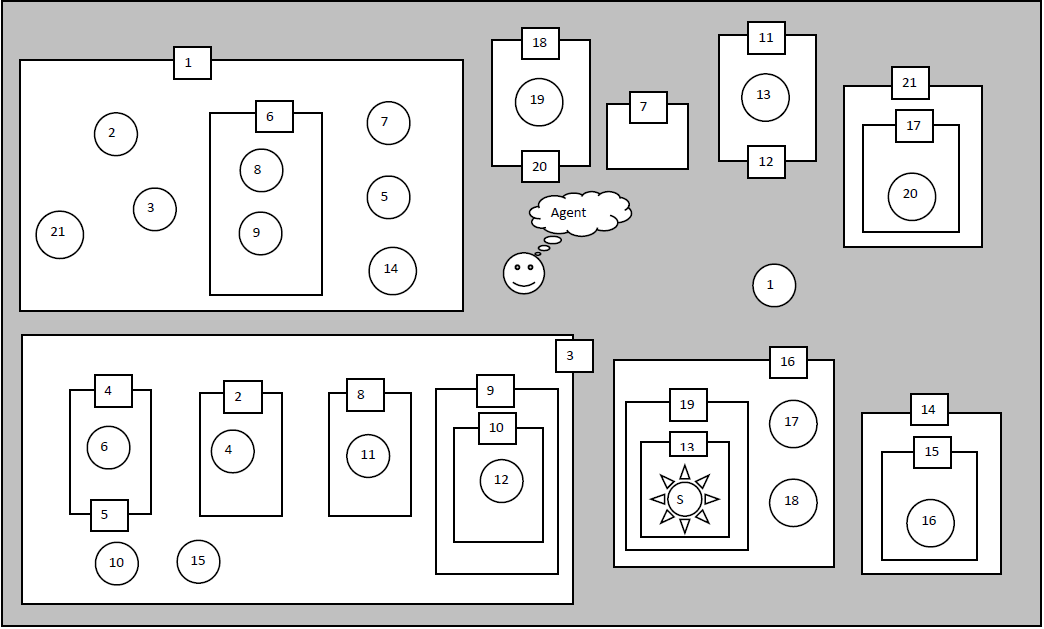
\includegraphics[width=1\textwidth]{content/pictures/situation.png}
        \caption{Ausgangslage}
        \label{fig:situation}
    \end{center}
\end{figure}

\section{Aufgabenstellung}
Folgende Aufgaben gibt es zu lösen in diesem Projekt:
\begin{itemize}
    \item Schreiben Sie ein Prolog-Programm, das unsere obige Problemsituation modellieren unter Annahme, 
    dass die vollständige Information gegeben ist. Es soll möglich sein, mittels Anfragen zu 
    überprüfen, ob eine bestimmte Türe erreichbar ist oder ob ein bestimmter Raum betreten 
    werden kann, usw.
    \item Modellieren Sie unter Verwendung von Listen die Möglichkeit einen Handlungsplan zu erhalten, 
    der aufzeigt, wie die einzelnen Ziele erreicht werden können.
\end{itemize}
\newpage

